%=============================================================================
%  PROJECT REPORT — full technical report with table of contents
%  Plain black text on white. No coloured boxes, no shaded panels.
%  Compile:  pdflatex project_report.tex   (run twice for the contents page)
%=============================================================================
\documentclass[11pt,a4paper]{report}

\usepackage[T1]{fontenc}
\usepackage[utf8]{inputenc}
\usepackage{mathptmx}                 % Times-like serif: standard for reports
\usepackage[scaled=0.88]{helvet}      % sans for headings only
\usepackage{courier}
\usepackage[margin=1in,top=1.1in,bottom=1.1in]{geometry}
\usepackage{graphicx}
\usepackage{booktabs}
\usepackage{amsmath,amssymb}
\usepackage{tikz}
\usetikzlibrary{arrows.meta,positioning,calc}
\usepackage{titlesec}
\usepackage{tocloft}
\usepackage{fancyhdr}
\usepackage{caption}
\usepackage{enumitem}
\usepackage[hidelinks]{hyperref}

% ---- typography -------------------------------------------------------------
\linespread{1.08}
\setlength{\parskip}{0.45em}
\setlength{\parindent}{0pt}
\captionsetup{font=small,labelfont=bf,justification=raggedright,
              singlelinecheck=false}

% Headings: sans, no rules, no boxes
\titleformat{\chapter}[display]
  {\normalfont\sffamily\LARGE\bfseries}
  {\normalfont\sffamily\normalsize\MakeUppercase{\chaptertitlename\ \thechapter}}
  {6pt}{\Large}
\titlespacing*{\chapter}{0pt}{-16pt}{22pt}

\titleformat{\section}{\normalfont\sffamily\large\bfseries}{\thesection}{0.7em}{}
\titleformat{\subsection}{\normalfont\sffamily\normalsize\bfseries}{\thesubsection}{0.7em}{}
\titlespacing*{\section}{0pt}{14pt}{5pt}
\titlespacing*{\subsection}{0pt}{11pt}{4pt}

% Contents page: dotted leaders, no colour
\renewcommand{\cfttoctitlefont}{\sffamily\LARGE\bfseries}
\renewcommand{\cftchapfont}{\sffamily\bfseries}
\renewcommand{\cftchappagefont}{\sffamily\bfseries}
\renewcommand{\cftchapleader}{\cftdotfill{\cftdotsep}}
\setlength{\cftbeforechapskip}{6pt}

% Running head: plain rule only
\pagestyle{fancy}
\fancyhf{}
\renewcommand{\headrulewidth}{0.4pt}
\fancyhead[L]{\footnotesize\sffamily ADAS Perception Pipeline}
\fancyhead[R]{\footnotesize\sffamily\thepage}

\begin{document}

%=============================================================================
% TITLE PAGE
%=============================================================================
\begin{titlepage}
\centering
\vspace*{2.2cm}

{\sffamily\Large PROJECT REPORT\par}
\vspace{1.4cm}

{\sffamily\huge\bfseries A Fail-Safe Monocular Perception\\[0.25em]
Pipeline for Collision and Overtaking\\[0.25em]
Decisions in Unstructured Traffic\par}

\vspace{1.6cm}
\rule{0.55\textwidth}{0.4pt}
\vspace{1.6cm}

{\large Submitted by\par}
\vspace{0.5em}
{\large\bfseries Krish Manwani \quad\textbullet\quad Vishal Bansal\par}

\vspace{1.4cm}
{\large Under the guidance of\par}
\vspace{0.5em}
{\large\bfseries Pranshu Chander \quad\textbullet\quad Bhushan Singh Negi\par}

\vspace{2.4cm}
{\large IBM Internship\par}
\vspace{0.35em}
{\large 2026\par}

\vfill
{\footnotesize All results reported in this document are measured from
executed runs. Sections carrying unmeasured values are marked explicitly.\par}
\end{titlepage}

%=============================================================================
\pagenumbering{roman}
\setcounter{page}{1}

\tableofcontents
\clearpage
\listoffigures
\vspace{1.5em}
\listoftables
\clearpage

%=============================================================================
\chapter*{Abstract}
\addcontentsline{toc}{chapter}{Abstract}
\markboth{Abstract}{}

Driver-assistance systems developed against Western and East Asian benchmarks
degrade on unstructured roads, where lane markings are intermittent and the
vehicle population includes categories those benchmarks never recorded. This
report documents a six-stage monocular camera perception pipeline that performs
object detection, multi-object tracking, lane and drivable-corridor estimation,
metric depth recovery, time-to-collision computation, and an overtaking safety
verdict in a single forward pass per frame.

Two design commitments distinguish the system. First, every stage substitutes a
weaker method rather than aborting when a model or weight file is unavailable —
a property verified in deployment when the lane network failed to initialise and
the pipeline nonetheless completed all 3{,}604 frames of the evaluation sequence.
Second, quantities informing safety decisions are expressed in physical units:
closing speed is differentiated from metric depth rather than image-plane
motion, and lane curvature is projected onto the ground plane so the resulting
radius can be compared against road-geometry design standards instead of an
uncalibrated pixel threshold.

On a merged validation split of 1{,}496 images containing 8{,}104 annotated
instances the detector attains 95.4\,\% mAP@0.5 and 79.9\,\% mAP@0.5:0.95, with
infrequent classes matching or exceeding the aggregate figure. The complete
pipeline sustains 23.1 frames per second on an NVIDIA H100 accelerator. A
geometric plausibility filter removes detections whose implied physical size is
inconsistent with their measured depth, rejecting 13.8\,\% of size-checked
candidates. The report states the system's untrained capabilities explicitly and
traces each to a data deficiency rather than an implementation defect.

\clearpage
\pagenumbering{arabic}
\setcounter{page}{1}

%=============================================================================
\chapter{Introduction}

\section{Background}

Perception stacks for driver assistance are overwhelmingly developed against a
small family of benchmarks. KITTI~\cite{geiger2012kitti} dominates object
detection and CULane~\cite{pan2018scnn} dominates lane estimation. Both were
recorded where traffic is lane-disciplined, markings are continuous, and the set
of vehicle types is small and homogeneous.

Systems tuned on this material transfer poorly to roads that violate those
premises. Varma \textit{et al.}~\cite{varma2019idd} documented the discrepancy
quantitatively, observing that segmentation models trained on structured-road
corpora score substantially lower on Indian road scenes than on their native
distribution.

\section{Problem Statement}

The degradation is not uniform. It manifests as three distinct failure modes,
each requiring a different remedy — a distinction that matters, because
treating all three as one problem leads to the wrong fix being applied.

\subsection{Category omission}

A detector whose label space lacks a class cannot abstain from it; it assigns
the nearest available label. A three-wheeled passenger vehicle becomes a car; a
hand-cart becomes miscellaneous clutter. Downstream logic then reasons about an
object whose dimensions and kinematics it has fundamentally misjudged. This is
more hazardous than a missed detection, because the system acts with confidence
on a wrong premise.

\subsection{An absent estimation target}

Lane-line detectors regress a curve through painted markings. Where the paint is
faded, absent, or disregarded by traffic, the quantity being estimated does not
exist in the scene. Retraining the lane model cannot repair this: the deficiency
lies in the scene, not the estimator.

\subsection{Spurious activation}

Under distribution shift a detector's confidence becomes a less faithful
indicator of correctness. Boxes appear on painted advertisements, shopfront
imagery, and specular reflections — objects with no physical extent at all.

\section{Objectives}

\begin{enumerate}[leftmargin=1.6em,itemsep=2pt]
  \item Build a single-pass perception pipeline producing two actionable driver
        outputs: an imminent-collision alert and an overtaking verdict.
  \item Ensure each stage degrades to a weaker method rather than terminating
        the pipeline when a component is unavailable.
  \item Express safety-relevant quantities in physical units rather than image
        units, so thresholds refer to external standards.
  \item Suppress spurious detections using geometric consistency rather than
        confidence thresholding alone.
  \item Evaluate end to end and report untrained capabilities explicitly.
\end{enumerate}

\section{Scope and Non-Goals}

The system is camera-only. Active range sensing would yield more reliable
distances, and the monocular choice should be read as a deployability
trade-off rather than a claim of superiority. The system is a perception and
advisory layer; it issues no control commands.

%=============================================================================
\chapter{Literature Review}

\section{The Domain-Shift Problem}

The India Driving Dataset~\cite{varma2019idd} established that benchmarks
recorded in countries with well-developed road infrastructure do not transfer
directly to unstructured traffic. It introduced an expanded label hierarchy and,
notably, explicit \textit{fallback} categories for road regions and vehicles
that structured taxonomies cannot express. The authors' framing of the problem
is the foundation of this project:

\begin{quote}
\small
Datasets like KITTI, Cityscapes, Argoverse, and nuScenes are captured in
developed countries where infrastructure is well-developed and road activity is
structured\ldots results obtained from these datasets are often not directly
applicable in unstructured road situations prevalent in large parts of the
world.\par
\hfill\textit{— Varma et al., WACV 2019}
\end{quote}

Subsequent corpora reinforced the finding at larger scale.
DriveIndia~\cite{kumar2025driveindia} contributes 66{,}986 annotated images
spanning 24 traffic categories collected over more than 3{,}400\,km of driving,
reporting a best mAP@0.5 of 78.7\,\% among YOLO-family baselines. The UVH-26
release~\cite{iisc2025uvh26} contributes 26{,}646 traffic-camera images with 14
India-specific vehicle classes and reports improvements of up to 31.5\,\% in
mAP@0.5:0.95 for detectors fine-tuned on this material relative to COCO-trained
initialisations. Together these establish both that the gap is substantial and
that supervised adaptation closes a large fraction of it.

\section{Component Architectures}

\subsection{Object detection}

Single-stage detection descends from the reformulation of detection as direct
regression introduced by Redmon \textit{et al.}~\cite{redmon2016yolo}. This work
adopts the YOLO11 implementation~\cite{ultralytics2024yolo11}, whose anchor-free
head and decoupled classification and regression branches provide a favourable
accuracy-to-latency ratio at the input resolution the latency budget permits.

\subsection{Lane estimation}

CLRNet~\cite{zheng2022clrnet} detects lane candidates from high-level semantic
features and refines them against lower-level detail, introducing a line-based
intersection-over-union objective that regresses each lane as a unit rather than
as independent points. It is reported to perform particularly well on curved and
nocturnal subsets — the conditions of greatest interest here. Ultra-Fast Lane
Detection v2~\cite{qin2024ufldv2}, which formulates lane localisation as
hybrid-anchor ordinal classification, is retained as a lower-latency
alternative.

\subsection{Multi-object tracking}

ByteTrack~\cite{zhang2022bytetrack} observes that low-confidence detections
frequently correspond to genuine but occluded objects, and matches them against
unmatched tracks in a second association stage. Continuity of identity is a
precondition for the temporal differencing the collision estimate depends on.

\subsection{Monocular depth}

Depth Anything V2~\cite{yang2024depthv2} provides a metric-calibrated outdoor
variant returning absolute distances, removing the scale ambiguity that would
otherwise prevent a monocular system from reporting time-to-collision in
seconds.

\subsection{Low-light enhancement}

The zero-reference curve estimation of Li \textit{et al.}~\cite{li2021zerodce}
requires no paired day--night supervision, which suits a project without access
to registered night-time ground truth.

\section{Consistency and Reliability}

The plausibility filter developed in this work follows the observation from the
monocular 3D detection literature~\cite{lian2022geoconsistency} that detectors
are susceptible to inconsistency between an object's apparent size and its
estimated depth, and that enforcing agreement between the two is an effective
corrective. The principle is applied here at the level of detection admission
rather than 3D box regression.

\section{Synthesis: What the Survey Determined}

Table~\ref{tab:litmap} records how each finding translated into a concrete
design decision. This mapping is the substantive output of the review.

\begin{table}[t]
\caption{Findings from the literature and the design decisions they produced}
\label{tab:litmap}
\small
\begin{tabular}{p{0.46\textwidth}p{0.46\textwidth}}
\toprule
\textbf{Finding} & \textbf{Design consequence} \\
\midrule
Western and East Asian benchmarks do not transfer to unstructured roads
  & Label space extended from 11 to 15 categories; converters built for three
    Indian corpora \\
\addlinespace
COCO-trained detectors miss three-wheelers and light commercial vehicles
entirely
  & The observed failure was attributed to data rather than implementation,
    redirecting effort accordingly \\
\addlinespace
Sequential fine-tuning risks forgetting the original categories
  & Corpora merged and trained jointly rather than in sequence \\
\addlinespace
Fine-tuning on Indian data yields up to $+31.5$ points mAP@0.5:0.95
  & Adopted as the measurable target for the adaptation experiment \\
\addlinespace
Detectors hallucinate objects under distribution shift
  & Geometric plausibility filter added, rather than raising the confidence
    threshold alone \\
\addlinespace
Apparent size and estimated depth must agree for a detection to be physical
  & That agreement test is the filter's mechanism \\
\addlinespace
Unstructured roads require drivable-region segmentation, not lane lines
  & Segmentation fallback that activates automatically \\
\bottomrule
\end{tabular}
\end{table}

\section{Research Gaps}

\begin{enumerate}[leftmargin=1.6em,itemsep=3pt]
  \item Benchmark corpora encode structured roads; transfer to unstructured
        traffic is poor and quantified only for isolated tasks, not for a full
        decision-producing pipeline.
  \item Lane-line estimation is undefined where markings are absent; the ground
        truth itself does not exist.
  \item Spurious detections under distribution shift are typically addressed by
        confidence thresholding, which trades recall for precision rather than
        testing physical plausibility.
  \item Curvature reported in pixels has no fixed physical meaning, yet is used
        to inform safety decisions.
  \item Published systems address these problems in isolation; none combines
        detection, tracking, lanes, depth, and two decision layers under an
        explicit degradation contract.
\end{enumerate}

%=============================================================================
\chapter{System Architecture}

\section{Overview}

Six stages execute in sequence on every frame. Each consumes the frame together
with the outputs of the stages above it; no second pass over the sequence is
required. Figure~\ref{fig:arch} presents the flow.

\begin{figure}[p]
\centering
\vspace*{1.2cm}
\begin{tikzpicture}[
  font=\small,
  node distance=0pt,
  every node/.style={align=left},
  stagehead/.style={font=\sffamily\bfseries\large},
  detail/.style={font=\small},
  stageout/.style={font=\small\itshape}
]

\def\W{14.6cm}

% One stage row: number | title, model, output — closed by a hairline.
\newcommand{\stagerow}[5]{%
  % #1 y-position  #2 number  #3 title  #4 model  #5 output
  \node[anchor=north west, stagehead] at (0,#1) {#2};
  \node[anchor=north west, stagehead] at (1.35,#1) {#3};
  \node[anchor=north west, detail]    at (1.35,#1-0.56) {#4};
  \node[anchor=north west, stageout]  at (1.35,#1-1.00) {#5};
  % Rule sits clear of the italic output line's descenders.
  \draw[gray!55, line width=0.3pt] (0,#1-1.50) -- (\W,#1-1.50);
}

% top rule + input
\draw[line width=0.8pt] (0,0.70) -- (\W,0.70);
\node[anchor=north west, font=\sffamily\bfseries\large] at (0,0.52) {INPUT};
\node[anchor=north west, detail] at (2.9,0.47)
     {monocular forward camera --- video file, image sequence, or live stream};
\draw[line width=0.8pt] (0,-0.18) -- (\W,-0.18);

\stagerow{-0.52}{0}{Scene lighting}
  {Zero-DCE++, CLAHE fallback}
  {$\rightarrow$\; enhanced frame, lighting state}

\stagerow{-2.14}{1}{Object detection}
  {YOLO11x at 640\,px}
  {$\rightarrow$\; boxes, class, confidence}

\stagerow{-3.76}{1b}{Plausibility filter}
  {depth--size consistency, pinhole model}
  {$\rightarrow$\; physically admissible detections}

\stagerow{-5.38}{2}{Lane and corridor}
  {CLRNet ResNet-101; surface segmentation fallback}
  {$\rightarrow$\; lane polylines, ego-lane boundaries}

\stagerow{-7.00}{3}{Multi-object tracking}
  {two-stage IoU association, smoothed velocity}
  {$\rightarrow$\; persistent identifiers, velocity}

\stagerow{-8.62}{4}{Metric depth and TTC}
  {Depth Anything V2, metric outdoor}
  {$\rightarrow$\; distance, closing speed, TTC, alert tier}

\stagerow{-10.24}{5}{Overtaking verdict}
  {five-rule conjunctive fusion, no learned component}
  {$\rightarrow$\; permitted / not permitted, with cause}

% output
\node[anchor=north west, font=\sffamily\bfseries\large] at (0,-11.98) {OUTPUT};
\node[anchor=north west, detail] at (2.9,-12.03)
     {annotated video and a per-frame decision record};
\draw[line width=0.8pt] (0,-12.74) -- (\W,-12.74);

% flow spine on the left
\draw[-{Latex[length=2.4mm]}, gray!70, line width=0.6pt]
      (-0.55,0.40) -- (-0.55,-12.42);

\end{tikzpicture}
\vspace{0.5cm}
\caption[Six-stage pipeline architecture]{The six-stage pipeline. Stages run in
order on every frame, each consuming the outputs above it. Every stage
substitutes a weaker method rather than aborting when its model is
unavailable.}
\label{fig:arch}
\end{figure}

\section{Stage Descriptions}

\textbf{Stage 0 — Scene lighting.} Classifies illumination from the frame's own
intensity statistics and enhances only when the scene is genuinely dark, so
daytime sequences incur no cost.

\textbf{Stage 1 — Object detection.} Detects road users at 640\,px input
resolution.

\textbf{Stage 1b — Plausibility filter.} Removes physically impossible
candidates, as described in Section~\ref{sec:filter}.

\textbf{Stage 2 — Lane and corridor.} Estimates lane geometry, or the drivable
corridor where markings are unusable.

\textbf{Stage 3 — Tracking.} Associates detections across frames and maintains
smoothed velocity.

\textbf{Stage 4 — Depth and collision.} Recovers metric depth and derives
collision estimates.

\textbf{Stage 5 — Overtaking verdict.} Fuses the preceding outputs into a
permitted / not-permitted decision.

\section{Degradation Contract}

Every optional component is constructed inside a guarded initialiser. Failure to
load leaves the corresponding capability disabled and is reported at start-up,
but does not propagate. Consumers of an unavailable output fall back to a weaker
but valid estimate.

This is not a defensive convenience. It was exercised in deployment when the
lane network failed to initialise owing to a library incompatibility, and the
pipeline completed the full 3{,}604-frame sequence using the drivable-corridor
substitute.

%=============================================================================
\chapter{Methodology}

\section{Collision Estimation from Metric Depth}

An object's growth in the image plane is not equivalent to its approach in the
world; scale change confounds relative motion with lateral displacement and
camera pitch. Closing speed is therefore derived from depth rather than pixel
kinematics.

For a track $i$, distance $d_i$ is the median depth over the lower half of the
bounding box — the region corresponding to the object's contact with the road
surface. The upper half is excluded because glazing and reflective bodywork
corrupt monocular depth there. The median is preferred to the mean for
resistance to outlying pixels.

Maintaining a bounded history of $d_i$, the closing speed over $n$ frames at
frame rate $f$ is
\begin{equation}
  v_i = \frac{d_i^{(t-n)} - d_i^{(t)}}{n/f},
\end{equation}
positive when approaching, and the time-to-collision is
\begin{equation}
  \tau_i = \frac{d_i^{(t)}}{v_i}, \qquad v_i > v_{\min}.
\end{equation}

The threshold $v_{\min}$ suppresses alerts on objects whose apparent approach is
attributable to depth noise. Alerts are emitted at two severities and only for
objects within the ego corridor, so oncoming and roadside traffic does not
generate spurious warnings. Distance history is nevertheless maintained for
\textit{all} tracks, including those outside the corridor, because the
overtaking stage requires the closing speed of oncoming vehicles.

\section{Plausibility Filtering}
\label{sec:filter}

Under the pinhole model, an object of image width $w_{\mathrm{px}}$ at depth $d$
observed with focal length $f_{\mathrm{px}}$ subtends a physical width
\begin{equation}
  W = \frac{w_{\mathrm{px}}\, d}{f_{\mathrm{px}}}.
\end{equation}

For each class an admissible interval $[W_{\min}, W_{\max}]$ is defined, and
candidates whose implied $W$ falls outside it after a multiplicative tolerance
are discarded. A detection fired on printed imagery or a reflection has no
consistent depth signature at its apparent scale and is removed, whereas a
genuine vehicle satisfies the relation. Classes of genuinely unbounded extent
are exempted rather than forced into an arbitrary interval.

Where the camera is uncalibrated, $f_{\mathrm{px}}$ must be estimated from an
assumed field of view. Because such an estimate can err in either direction, the
tolerance is \textit{widened} in the uncalibrated case. This asymmetry is
deliberate: discarding a real vehicle is more consequential than admitting a
spurious one, since spurious detections remain subject to the ego-corridor test
before they can raise an alert. Supplying a calibration restores the narrow
interval automatically.

\section{Curvature in Physical Units}

Curvature computed on image-plane polylines has no fixed physical
interpretation: it varies with sensor resolution, focal length, and mounting
geometry, so the same road yields different values on different vehicles.

A plane-induced homography~\cite{hartley2004multiple} projects lane points onto
the ground plane. A second-order polynomial $x = az^2 + bz + c$ is fitted in
ground coordinates, and
\begin{equation}
  \kappa = \frac{|2a|}{\left(1 + (2az_f + b)^2\right)^{3/2}}
\end{equation}
is evaluated at the furthest visible distance $z_f$, giving a radius
$R = 1/\kappa$ in metres. This admits comparison against minimum horizontal
curve radii from road-geometry design practice, so a verdict that a curve is too
tight for a safe overtaking manoeuvre rests on an external standard rather than
a tuned constant.

\section{Overtaking Verdict}

The verdict is a conjunction of five conditions, evaluated without a learned
component:

\begin{enumerate}[leftmargin=1.6em,itemsep=1pt]
  \item marking legality,
  \item curve radius,
  \item visibility,
  \item oncoming traffic within the manoeuvre window,
  \item clear distance ahead of the lead vehicle.
\end{enumerate}

All five must hold. Any input that is missing or uncertain resolves to
\textit{not permitted}. The module is conservative by construction, which is the
correct property for a manoeuvre that places the vehicle in an opposing lane.

%=============================================================================
\chapter{Data Pipeline and Experimental Setup}

\section{Preprocessing}

Source annotations were converted to a common normalised format and remapped
onto a unified label space so that corpora with differing taxonomies could be
combined. Boxes smaller than two pixels in either dimension were discarded and
all coordinates clipped to the image. The checkpoint evaluated here was trained
on 5{,}985 images with 1{,}496 held out for validation.

Augmentation comprised mosaic composition, MixUp, copy--paste, HSV value jitter,
rotation to $\pm5^{\circ}$, translation, scaling, and horizontal flipping.

\section{Unified Label Space}

Fifteen categories, extended beyond a structured-road taxonomy with
\textit{autorickshaw}, \textit{animal}, \textit{rider}, and an open-world
\textit{vehicle fallback} class following the argument
of~\cite{varma2019idd}:

\begin{center}
\small
\begin{tabular}{llll}
0\; car & 4\; pedestrian & \;\;8\; traffic light & 12\; animal \\
1\; truck & 5\; cyclist & \;\;9\; traffic sign & 13\; rider \\
2\; bus & 6\; motorcycle & 10\; miscellaneous & 14\; vehicle fallback \\
3\; van & 7\; tram & & \\
\end{tabular}
\end{center}

As Chapter~\ref{ch:limits} discusses, the merge used for this checkpoint
exercised only a subset of these.

\section{Training Configuration}

AdamW with an initial learning rate of $5\times10^{-4}$ under a cosine schedule
with five warm-up epochs; batch size 16 at $640\times640$; mixed precision;
early stopping with patience 50. All experiments ran on a single NVIDIA H100
80\,GB accelerator on a PBS-scheduled cluster.

\section{Verification Procedure}

Because training occupies the accelerator for extended periods, the decision
logic — collision arithmetic, all five overtaking conditions, lane coordinate
mapping, plausibility filtering, and the degradation contract — is exercised
against synthetic inputs by a 62-check suite requiring no accelerator, trained
weights, or dataset. It completes in seconds and is executed before any job is
queued.

The suite detected several defects, including two that had already reached the
cluster: a coordinate-space error in which lane predictions expressed in the
lane model's native resolution were applied directly to frames of a different
resolution, and an over-broad exception boundary that allowed an optional
component's failure to terminate the pipeline.

%=============================================================================
\chapter{Results}

\section{Detection Accuracy}

Table~\ref{tab:perclass} reports per-class performance on the held-out split.
Aggregate accuracy is 95.4\,\% mAP@0.5 and 79.9\,\% mAP@0.5:0.95, at 95.4\,\%
precision and 92.5\,\% recall over 8{,}104 instances.

\begin{table}[h]
\caption{Per-class detection performance (1{,}496 validation images,
8{,}104 instances)}
\label{tab:perclass}
\centering
\small
\begin{tabular}{lrrrrr}
\toprule
Class & Instances & P (\%) & R (\%) & mAP@0.5 & mAP@0.5:0.95 \\
\midrule
Car            & 5{,}798 & 95.7 & 96.6 & 97.9 & 87.6 \\
Pedestrian     &    884 & 95.0 & 81.3 & 89.0 & 55.9 \\
Van            &    587 & 94.9 & 97.3 & 97.5 & 86.0 \\
Cyclist        &    313 & 94.3 & 88.2 & 92.7 & 71.0 \\
Truck          &    219 & 97.5 & 98.6 & 99.4 & 91.5 \\
Miscellaneous  &    194 & 95.1 & 92.3 & 94.3 & 80.8 \\
Tram           &    109 & 95.3 & 93.1 & 96.8 & 86.7 \\
\midrule
\textbf{All}   & \textbf{8{,}104} & \textbf{95.4} & \textbf{92.5}
               & \textbf{95.4} & \textbf{79.9} \\
\bottomrule
\end{tabular}
\end{table}

Two observations merit attention.

Accuracy on infrequent categories does not collapse. Truck (219 instances) and
tram (109) match or exceed the aggregate figure despite being roughly
twenty-five times rarer than car, indicating that the balancing and augmentation
strategy suppressed the long-tail degradation typically seen on such
distributions.

Pedestrian localisation is the weakest column at 55.9\,\% under the strict
metric, while precision remains at 95.0\,\%. Pedestrians are found reliably but
bounded less tightly than vehicles, which is attributable to greater pose
variability and more frequent partial occlusion.

\begin{figure}[h]
\centering
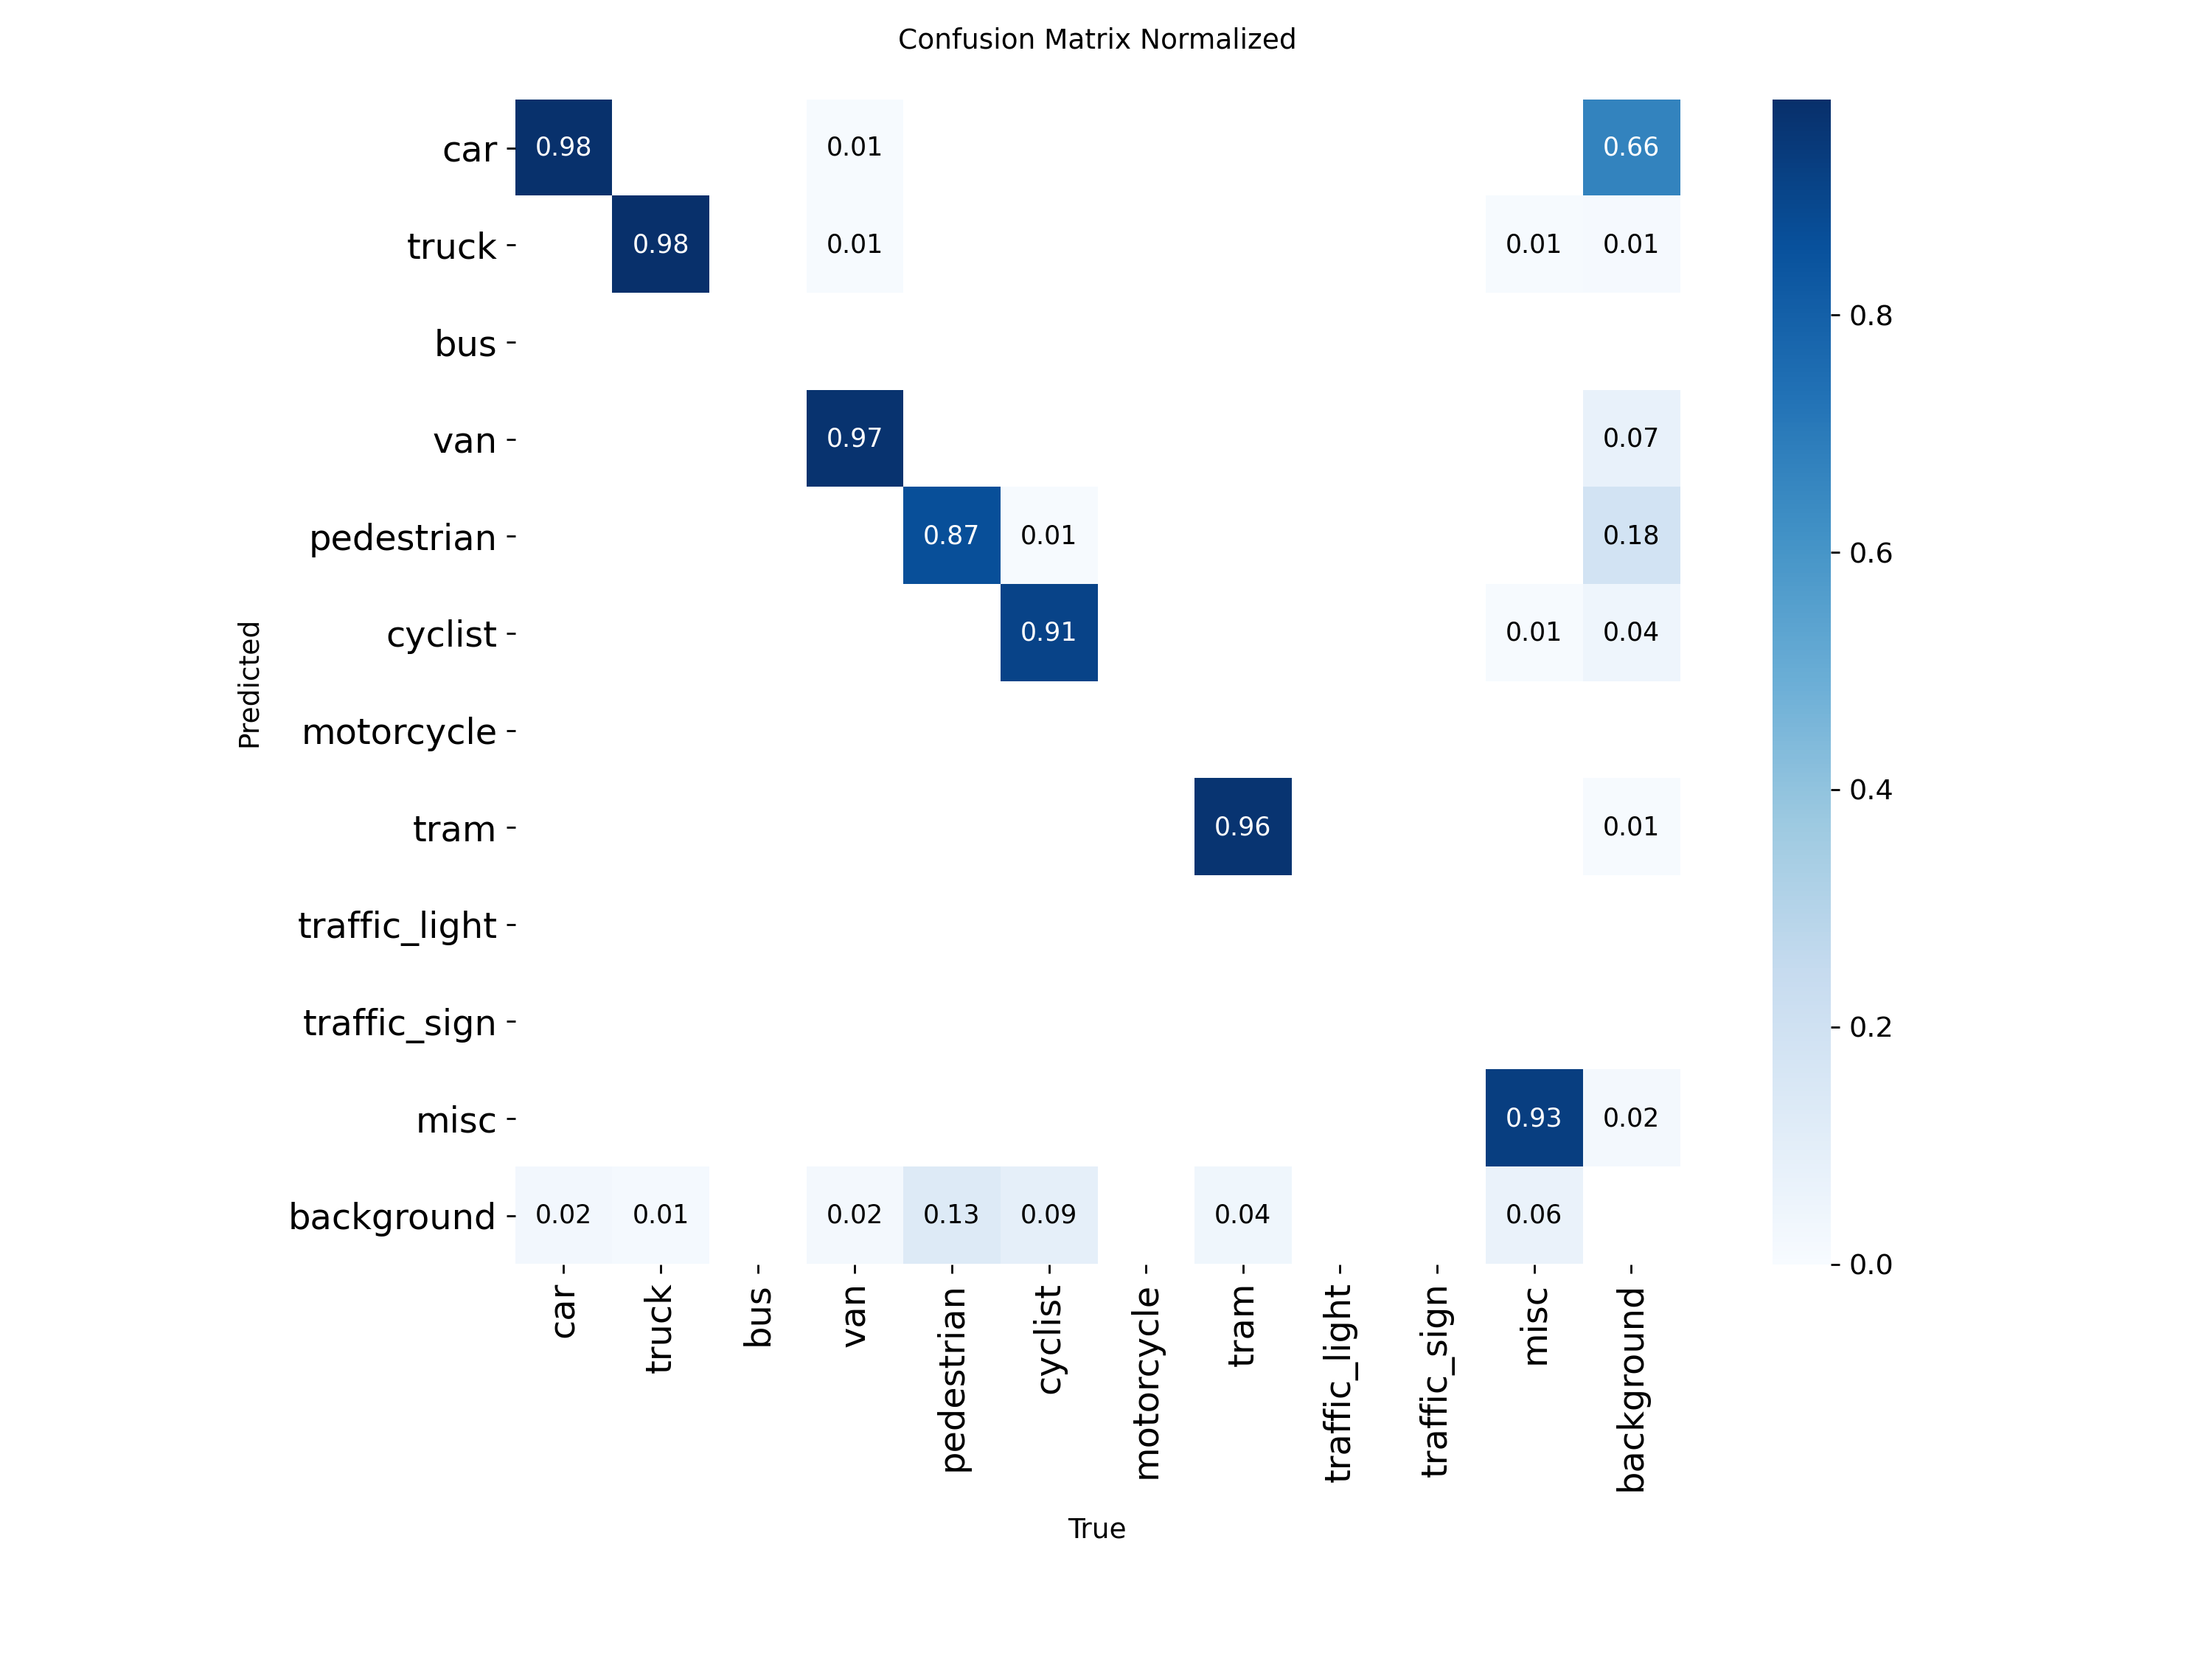
\includegraphics[width=0.72\textwidth]{figures/confusion_matrix_normalized.png}
\caption[Normalised confusion matrix]{Normalised confusion matrix on the
validation split. Diagonal entries are correct classifications; off-diagonal
entries show the categories most often interchanged.}
\label{fig:confusion}
\end{figure}

Residual confusion is concentrated between visually adjacent vehicle categories
rather than distributed arbitrarily, and the background row indicates that
missed detections rather than cross-class errors dominate the remaining loss.

\section{Effect of Training Schedule and Capacity}

Table~\ref{tab:progress} compares three configurations. Extending the medium
model from 50 to 500 epochs yields a larger improvement ($+2.5$ points mAP@0.5,
$+8.4$ points at the strict metric) than the subsequent increase in capacity
($+1.2$ and $+2.2$ points). Under a constrained accelerator budget, schedule
length was the more productive expenditure.

\begin{table}[h]
\caption{Effect of training schedule and model capacity}
\label{tab:progress}
\centering
\small
\begin{tabular}{llrrr}
\toprule
Configuration & Model & Epochs & mAP@0.5 & mAP@0.5:0.95 \\
\midrule
Baseline & YOLO11m & 50  & 91.7 & 69.3 \\
Extended & YOLO11m & 500 & 94.2 & 77.7 \\
\textbf{Final} & \textbf{YOLO11x} & \textbf{300} & \textbf{95.4} & \textbf{79.9} \\
\bottomrule
\end{tabular}
\end{table}

\begin{figure}[h]
\centering
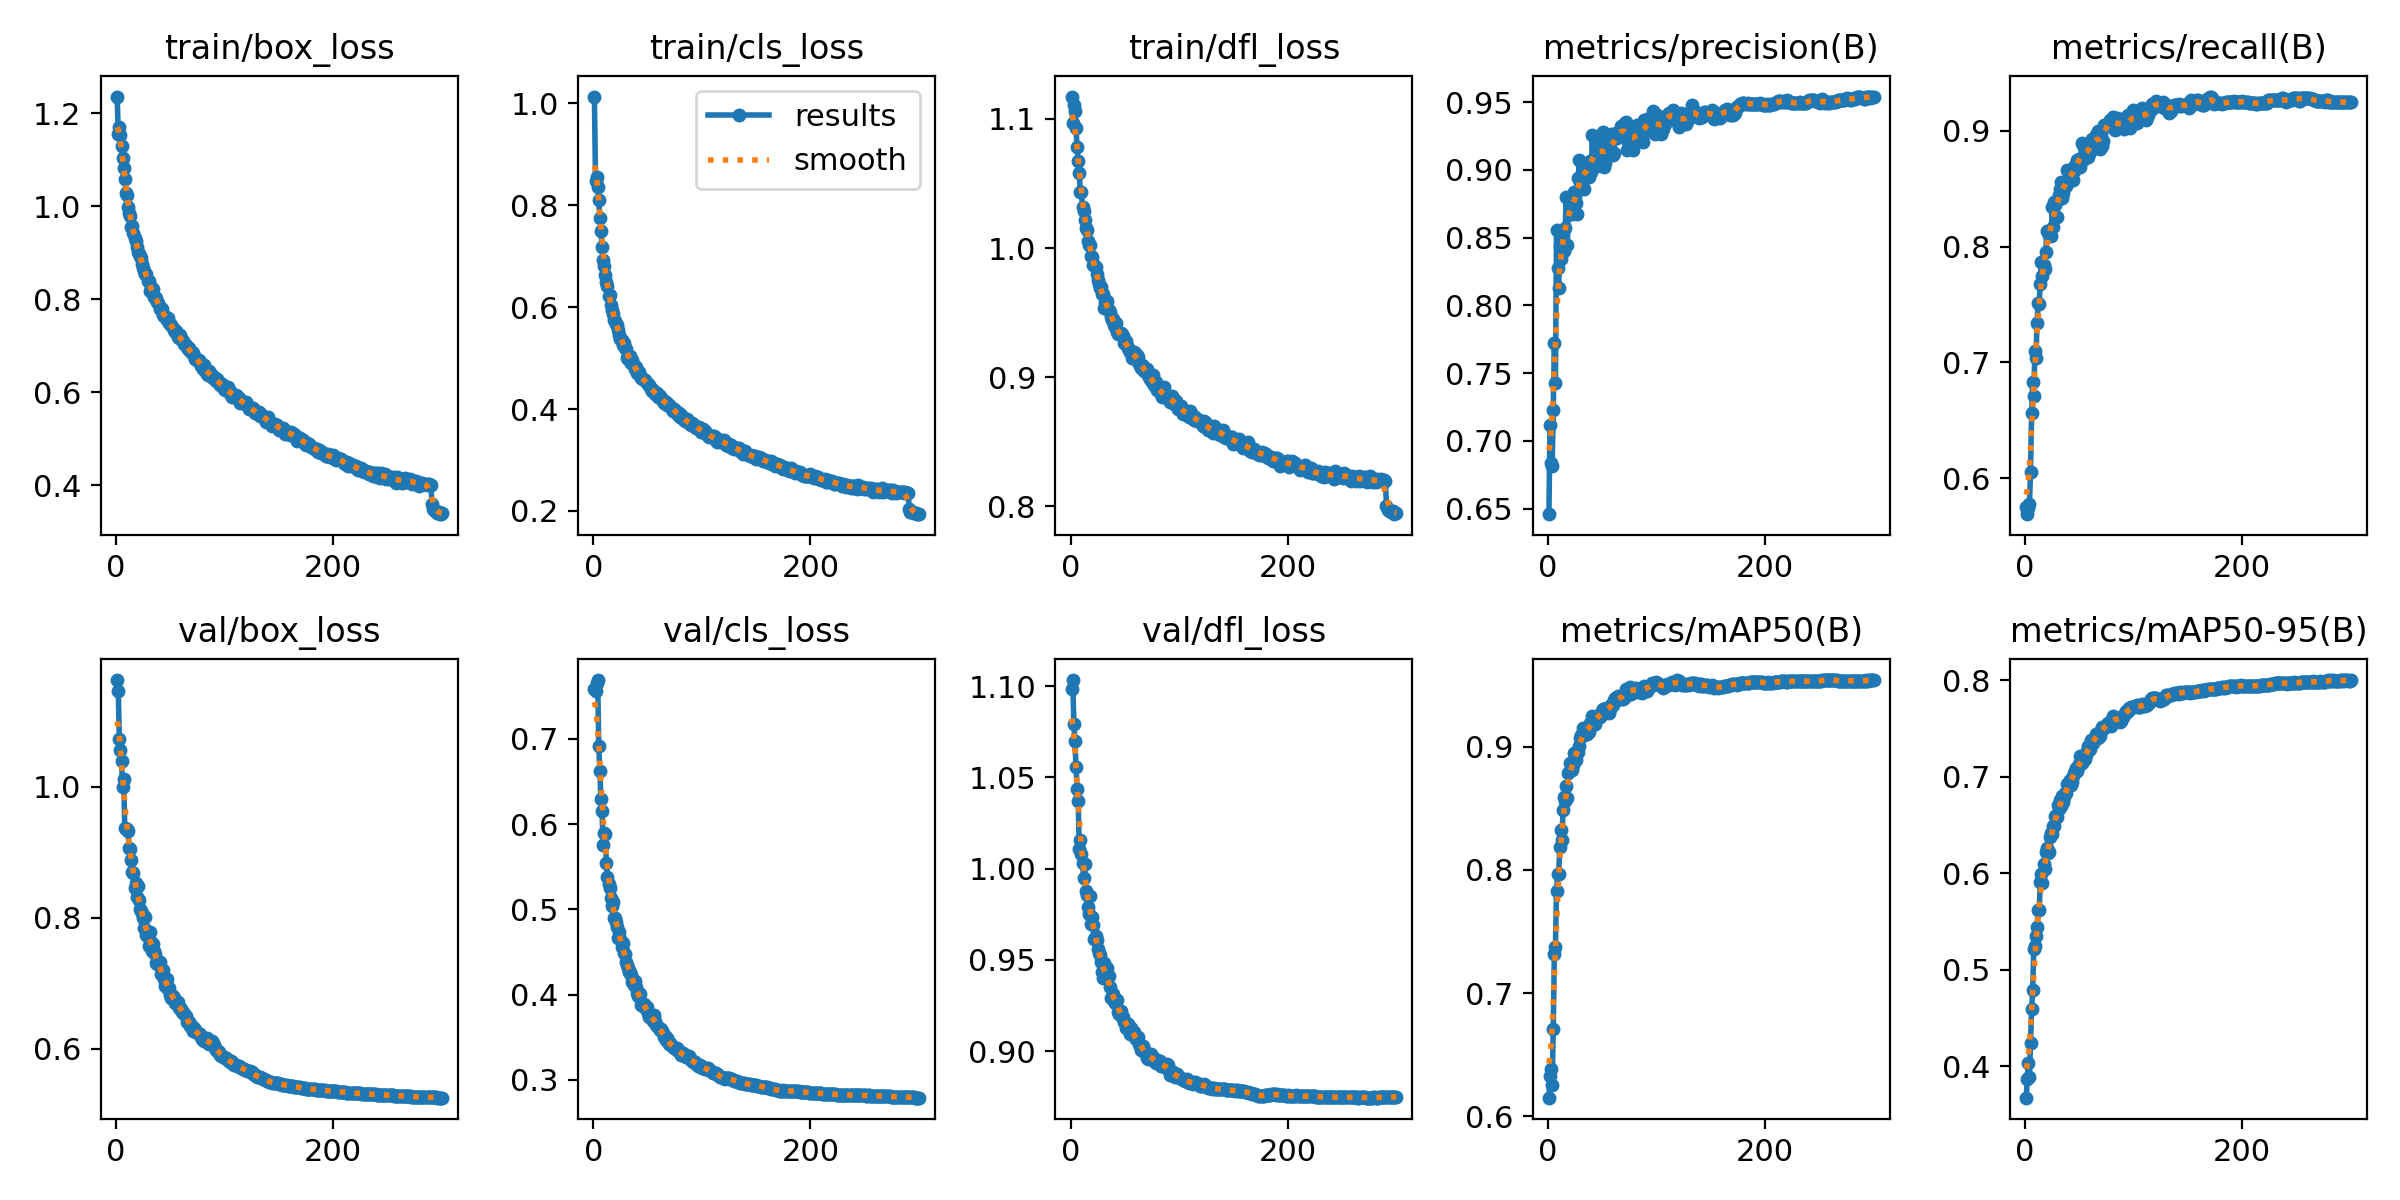
\includegraphics[width=0.95\textwidth]{figures/results.png}
\caption[Training curves]{Training behaviour of the final configuration. Box,
classification, and distribution-focal losses converge without divergence on
either split, and both mAP measures rise monotonically before flattening.}
\label{fig:training}
\end{figure}

\section{End-to-End Pipeline}

Table~\ref{tab:pipeline} summarises a complete run over a 3{,}604-frame road
sequence. All six stages sustain 23.1 frames per second at a mean latency of
43\,ms.

\begin{table}[h]
\caption{Complete pipeline over a 3{,}604-frame sequence}
\label{tab:pipeline}
\centering
\small
\begin{tabular}{lr}
\toprule
Measurement & Value \\
\midrule
Frames processed              & 3{,}604 \\
Throughput                    & 23.1 fps (43\,ms mean) \\
Collision alerts              & 69 (20 brake, 49 warning) \\
Frames with lane geometry     & 3{,}603 of 3{,}604 \\
Detections rejected by filter & 979 of 7{,}077 (13.8\,\%) \\
Detector parameters           & 56.8\,M (194.5 GFLOPs) \\
\bottomrule
\end{tabular}
\end{table}

An initial measurement of the same configuration returned 0.9 frames per second.
The cause was placement of the depth model on the host processor rather than any
property of the pipeline; on the accelerator the identical code is approximately
twenty-five times faster. This is recorded because the two figures separate a
deployable system from an unusable one while differing in no respect other than
device placement — a diagnosis worth making before attributing latency to
architecture.

\begin{figure}[h]
\centering
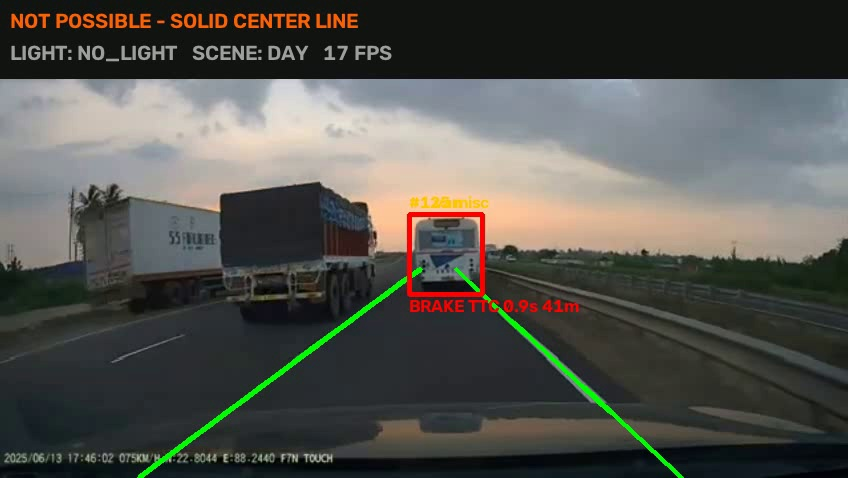
\includegraphics[width=0.47\textwidth]{figures/BRAKE_01021.jpg}\hfill
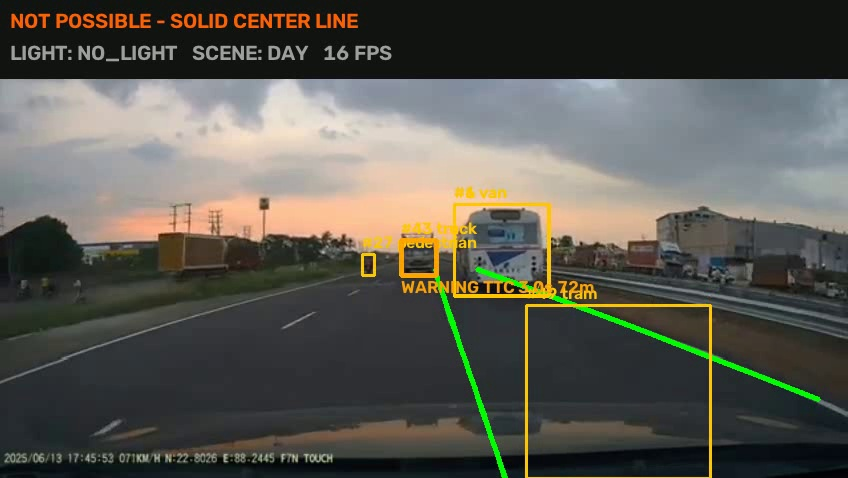
\includegraphics[width=0.47\textwidth]{figures/WARNING_00423.jpg}

\vspace{0.6em}
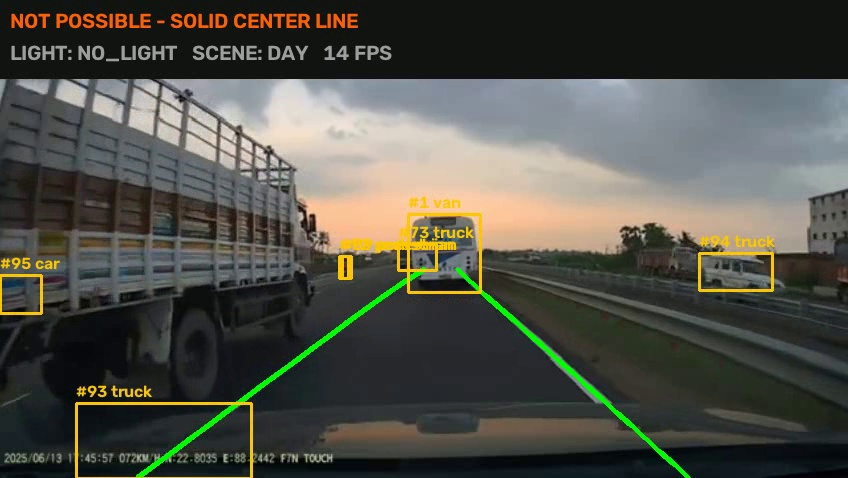
\includegraphics[width=0.72\textwidth]{figures/BUSY_00682.jpg}
\caption[Pipeline output on road footage]{Pipeline output. Left: a brake-tier
alert. Right: the warning tier. Below: simultaneous tracking under dense
traffic. Every overlay was produced by the pipeline; none was added
afterwards.}
\label{fig:qualitative}
\end{figure}

\section{Plausibility Filter}

The filter removed 979 of 7{,}077 size-checked candidates. In an earlier
configuration using a narrower tolerance under an uncalibrated focal length, the
rejection rate reached approximately 27\,\% and included large numbers of
vehicle classes, indicating suppression of genuine objects rather than spurious
ones. Widening the tolerance in the uncalibrated regime, as described in
Section~\ref{sec:filter}, reduced the rate to 13.8\,\%.

The episode illustrates the intended asymmetry: an uncertain calibration should
relax the admission criterion, not tighten it.

%=============================================================================
\chapter{Limitations}
\label{ch:limits}

Each limitation below traces to a data deficiency rather than an implementation
defect, and each therefore implies a different remedy.

\section{Four Declared Classes Carry No Training Examples}

The label space defines traffic lights, traffic signs, buses, and motorcycles,
but the merge that produced this checkpoint drew from a single structured-road
source containing none of them. Validation consequently reports seven classes
rather than eleven. No modification to the model can address this; a corpus
containing the categories is required.

\section{India-Specific Categories Are Defined but Untrained}

The autorickshaw, animal, rider, and fallback classes are present in the
taxonomy, and conversion pipelines for three Indian
corpora~\cite{varma2019idd,kumar2025driveindia,iisc2025uvh26} are implemented
and tested. The retraining that would populate these classes has not been
performed. Reported accuracy therefore reflects the structured-road distribution
and should not be read as performance on unstructured traffic.

\section{The Overtaking Verdict Is Conservative Without Marking Type}

Without a reliable solid-versus-broken classification, the legality condition
cannot be satisfied and the verdict remains \textit{not permitted}. This is the
intended fail-safe rather than a malfunction, but it does mean the module is
inactive on sequences lacking marking-type input.

\section{Monocular Depth Is Less Reliable Than Active Ranging}

Distance, and hence time-to-collision, inherits the error characteristics of
learned monocular depth. A system with an active range sensor would obtain more
dependable distances; the camera-only choice reflects a deployability constraint
and should be recognised as a trade-off.

%=============================================================================
\chapter{Conclusion and Future Work}

\section{Conclusion}

This report has presented a monocular perception pipeline integrating detection,
tracking, lane and corridor estimation, metric depth, and two decision layers
within a single pass, attaining 95.4\,\% mAP@0.5 and sustaining 23.1 frames per
second on an H100 accelerator.

The system's distinguishing commitments are a degradation contract exercised
under real deployment failure, and the expression of safety-relevant quantities
in physical rather than image units. Its limitations are stated with their
diagnosed causes rather than omitted.

\section{Future Work}

\begin{enumerate}[leftmargin=1.6em,itemsep=3pt]
  \item \textbf{Retraining on the merged Indian corpora.} The conversion
        infrastructure is complete. The improvement reported
        in~\cite{iisc2025uvh26} for comparable adaptation suggests the
        achievable magnitude. This is the highest-value next step.
  \item \textbf{Incorporating a corpus containing traffic lights and signs},
        rendering four presently untrainable classes trainable.
  \item \textbf{Camera calibration}, which would narrow the plausibility filter
        from its uncertainty-widened interval and supply metric curvature.
  \item \textbf{Supervised training of the drivable-corridor segmenter} to
        replace the present classical-vision substitute, improving lane
        estimation precisely where painted markings are unavailable.
\end{enumerate}

%=============================================================================
\begin{thebibliography}{99}
\addcontentsline{toc}{chapter}{References}

\bibitem{geiger2012kitti}
A.~Geiger, P.~Lenz, and R.~Urtasun, ``Are we ready for autonomous driving? The
KITTI vision benchmark suite,'' in \textit{Proc. IEEE Conf. Comput. Vis. Pattern
Recognit. (CVPR)}, Providence, RI, USA, Jun. 2012, pp.~3354--3361.

\bibitem{pan2018scnn}
X.~Pan, J.~Shi, P.~Luo, X.~Wang, and X.~Tang, ``Spatial as deep: Spatial CNN for
traffic scene understanding,'' in \textit{Proc. AAAI Conf. Artif. Intell.
(AAAI)}, New Orleans, LA, USA, Feb. 2018, pp.~7276--7283.

\bibitem{varma2019idd}
G.~Varma, A.~Subramanian, A.~Namboodiri, M.~Chandraker, and C.~V. Jawahar,
``IDD: A dataset for exploring problems of autonomous navigation in
unconstrained environments,'' in \textit{Proc. IEEE Winter Conf. Appl. Comput.
Vis. (WACV)}, Waikoloa Village, HI, USA, Jan. 2019, pp.~1743--1751.

\bibitem{kumar2025driveindia}
R.~Kumar, D.~S. Reddy, and P.~Rajalakshmi, ``DriveIndia: An object detection
dataset for diverse Indian traffic scenes,'' in \textit{Proc. IEEE Int. Conf.
Intell. Transp. Syst. (ITSC)}, 2025.

\bibitem{iisc2025uvh26}
Artificial Intelligence and Robotics Initiative (AIM), Indian Institute of
Science, ``The Urban Vision Hackathon dataset and models: Towards image
annotations and accurate vision models for Indian traffic,'' Tech.
Rep. UVH-26-v1.0, Bengaluru, India, Nov. 2025.

\bibitem{redmon2016yolo}
J.~Redmon, S.~Divvala, R.~Girshick, and A.~Farhadi, ``You only look once:
Unified, real-time object detection,'' in \textit{Proc. IEEE Conf. Comput. Vis.
Pattern Recognit. (CVPR)}, Las Vegas, NV, USA, Jun. 2016, pp.~779--788.

\bibitem{ultralytics2024yolo11}
G.~Jocher and J.~Qiu, ``Ultralytics YOLO11,'' software release, Ultralytics,
2024. [Online]. Available: \url{https://github.com/ultralytics/ultralytics}

\bibitem{zheng2022clrnet}
T.~Zheng, Y.~Huang, Y.~Liu, W.~Tang, Z.~Yang, D.~Cai, and X.~He, ``CLRNet: Cross
layer refinement network for lane detection,'' in \textit{Proc. IEEE/CVF Conf.
Comput. Vis. Pattern Recognit. (CVPR)}, New Orleans, LA, USA, Jun. 2022,
pp.~898--907.

\bibitem{qin2024ufldv2}
Z.~Qin, P.~Zhang, and X.~Li, ``Ultra fast deep lane detection with hybrid anchor
driven ordinal classification,'' \textit{IEEE Trans. Pattern Anal. Mach.
Intell.}, vol.~46, no.~5, pp.~2555--2568, May 2024.

\bibitem{zhang2022bytetrack}
Y.~Zhang, P.~Sun, Y.~Jiang, D.~Yu, F.~Weng, Z.~Yuan, P.~Luo, W.~Liu, and
X.~Wang, ``ByteTrack: Multi-object tracking by associating every detection
box,'' in \textit{Computer Vision --- ECCV 2022}, Lecture Notes in Computer
Science, vol.~13682. Cham, Switzerland: Springer, 2022, pp.~1--21.

\bibitem{yang2024depthv2}
L.~Yang, B.~Kang, Z.~Huang, Z.~Zhao, X.~Xu, J.~Feng, and H.~Zhao, ``Depth
Anything V2,'' in \textit{Advances in Neural Information Processing Systems
(NeurIPS)}, vol.~37, 2024.

\bibitem{li2021zerodce}
C.~Li, C.~Guo, and C.~C. Loy, ``Learning to enhance low-light image via
zero-reference deep curve estimation,'' \textit{IEEE Trans. Pattern Anal. Mach.
Intell.}, vol.~44, no.~8, pp.~4225--4238, Aug. 2022.

\bibitem{lian2022geoconsistency}
Q.~Lian, B.~Ye, R.~Xu, W.~Yao, and T.~Zhang, ``Exploring geometric consistency
for monocular 3D object detection,'' in \textit{Proc. IEEE/CVF Conf. Comput.
Vis. Pattern Recognit. (CVPR)}, New Orleans, LA, USA, Jun. 2022,
pp.~1685--1694.

\bibitem{hartley2004multiple}
R.~Hartley and A.~Zisserman, \textit{Multiple View Geometry in Computer Vision},
2nd~ed. Cambridge, U.K.: Cambridge Univ. Press, 2004.

\end{thebibliography}

\end{document}
